\documentclass[11pt]{article}
%Gummi|065|=)
\title{\textbf{EV2.7.Dise\~no de Modulaci\'on de Ancho de Pulso(PWM)}}
\author{Cervantes Mart\'inez Luis Osvaldo\\
		Sistemas Electronicos de Interfaz\\
		Martes, 22 de Octubre 2019}

\date{}
\usepackage{graphicx}
\usepackage[hidelinks]{hyperref}
\usepackage{color}
\begin{document}

\maketitle
\begin{figure}[htp]
\centering

\includegraphics[scale=0.45]{/home/osvaldo/Escritorio/EV.2.7/UPZMG.png}
\caption{UPZMG}
\label{}
\end{figure}

\pagebreak
\section{¿Qu\'e es Modulaci\'on de Ancho de Pulso (PWM)?}
La modulaci\'on de ancho de pulso (PWM, por sus siglas en ingl\'es) de una se\~nal es una t\'ecnica que logra producir el efecto de una se\~nal anal\'ogica sobre una carga, a partir de la variaci\'on de la frecuencia y ciclo de trabajo de una se\~nal digital. El ciclo de trabajo describe la cantidad de tiempo que la se\~nal est\'a en un estado l\'ogico alto, como un porcentaje del tiempo total que este toma para completar un ciclo completo. La frecuencia determina que tan r\'apido se completa un ciclo (por ejemplo: 1000 Hz corresponde a 1000 ciclos en un segundo), y por consiguiente que tan r\'apido se cambia entre los estados l\'ogicos alto y bajo. Al cambiar una se\~nal del estado alto a bajo a una tasa lo suficientemente r\'apida y con un cierto ciclo de trabajo, la salida parecer\'a comportarse como una se\~nal anal\'ogica constante cuanto esta est\'a siendo aplicada a alg\'un dispositivo.

\section{¿Para qu\'e se \'utiliza?}
Se\~nales de PWM son utilizadas comunmente en el control de aplicaciones. Su uso principal es el control de motores de corriente continua, aunque tambi\'en pueden ser utilizadas para controlar v\'alvulas, bombas, sistemas hidr\'aulicos, y algunos otros dispositivos mec\'anicos. La frecuencia a la cual la se\~nal de PWM se generar\'a, depender\'a de la aplicaci\'on y del tiempo de respuesta del sistema que est\'a siendo controlado. A continuaci\'on se muestran algunas aplicaciones y sus respectivas frecuencias:
\begin{itemize}
\item Calentar elementos o sistemas con tiempos de respuesta lentos: 10-100 Hz o superior.            
\item Motores eléctricos de corriente continua: 5-10 kHz o superior.
\item Fuentes de poder o amplificadores de audio: 20-200 kHz o superior.
\end{itemize}

\pagebreak
\section{T\'ecnicas de modulaci\'onescalares o PWM}

Se  usa  en  inversores  DC/AC monof\'asicos y trif\'asicos. Se basan en la comparaci\'on de una se\~nal de referencia  a  modular  y  una  se\~nal portadora  de  forma  triangular  o diente de sierra \ref{Figura 2}; la comparaci\'on generar\'a un tren de pulsos de ancho espec\'ifico que se utilizan en la conmutaci\'on del puente inversor. La relaci\'on entre la amplitud de la se\~nal portadora y la se\~nal de referencia se llama \textit{\'indice de modulaci\'on} y  se  representa  por  $m_a$ \ref{1},  donde  $A_r$ es la amplitud de la se\~nal de referencia y $A_c$ es la amplitud de la se\~nal portadora. El \'indice de modulaci\'on  permite  obtener tensi\'on variable a la salida del inversor.


\begin{equation}
m_a=\frac{A_r}{A_c}
\label{1}
\end{equation}\\

\begin{equation}
 m_f=\frac{F_r}{F_c}
\label{2}
 \end{equation}



La relaci\'on entre la frecuencia dela se\~nal portadora y la frecuencia de referencia  se  denomina  \textit {\'indice de frecuecia} y se representa por $m_f$ \ref{2}, idealmente $m_f$ debe ser mayor a 21  y  la  frecuencia  de  la  portadora m\'ultiplo de la frecuencia de la se\~nal de referencia. El \'indice de frecuencia determina la distorsi\'on arm\'onica de la se\~nal de salida la cual es una medida de su  contenido  arm\'onico. La variaci\'on de la se\~nal de referencia y la  secuencia  de  conmutaci\'on dan como  resultado  diferentes  t\'ecnicas de modulaci\'on PWM, cada una modifica la eficiencia de la conversi\'on,  las  p\'erdidas  por  conmutaci\'on en el puente inversor y la pureza de la se\~nal de salida.


\begin{figure}[htp]
\centering
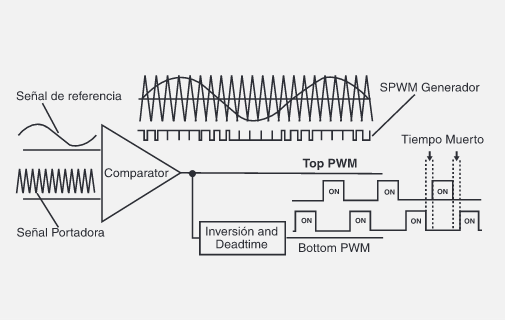
\includegraphics[scale=0.3]{/home/osvaldo/Escritorio/EV.2.7/Circuito generador escalar PWM.png}
\caption{Circuito generador escalar PWM}
\label{Figura 2}
\end{figure}
.

\pagebreak
\begin{thebibliography}{0}
\textcolor{blue}{\url{http://digital.ni.com/public.nsf/allkb/AA1BDEA4AA224E3E86257CE400707527}}\\

\textcolor{blue}{\url{https://www.redalyc.org/pdf/478/47802507.pdf}}


 \end{thebibliography}

\end{document}

